\documentclass{beamer}
\usepackage[utf8]{inputenc}

\title{Introduction to 3D vision}
\author{Timothée Wintz}\institute{Sony CSL Paris}

\graphicspath{{images}}

\begin{document}

\begin{frame}
\titlepage
\end{frame}

\section{Camera model}

\begin{frame}
    \tableofcontents
\end{frame}

\begin{frame}
    \tableofcontents[sectionstyle=show/shaded]
\end{frame}

\begin{frame}{Pinhole camera model}
    \centering
    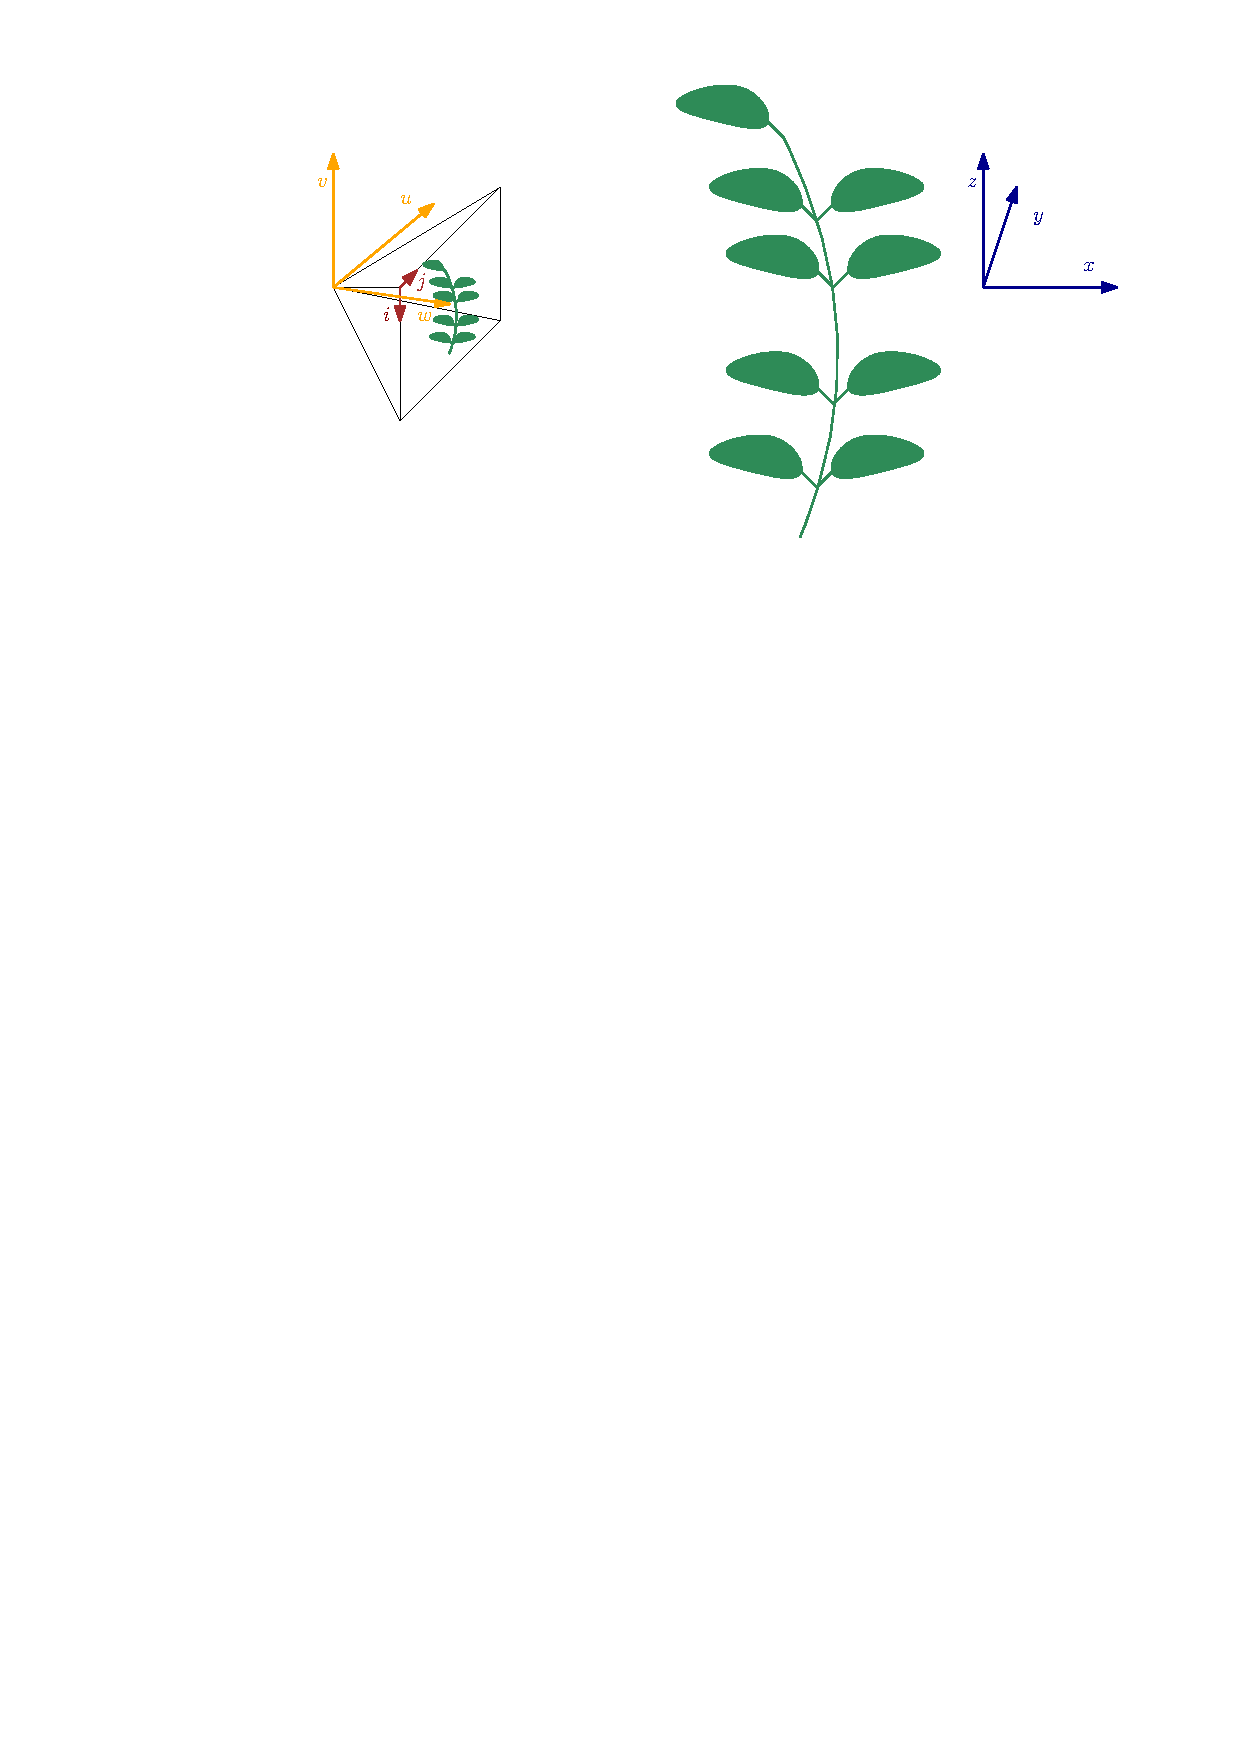
\includegraphics[width=\textwidth]{images/reperes.pdf}
\end{frame}

\begin{frame}{Camera pose}
    \centering
    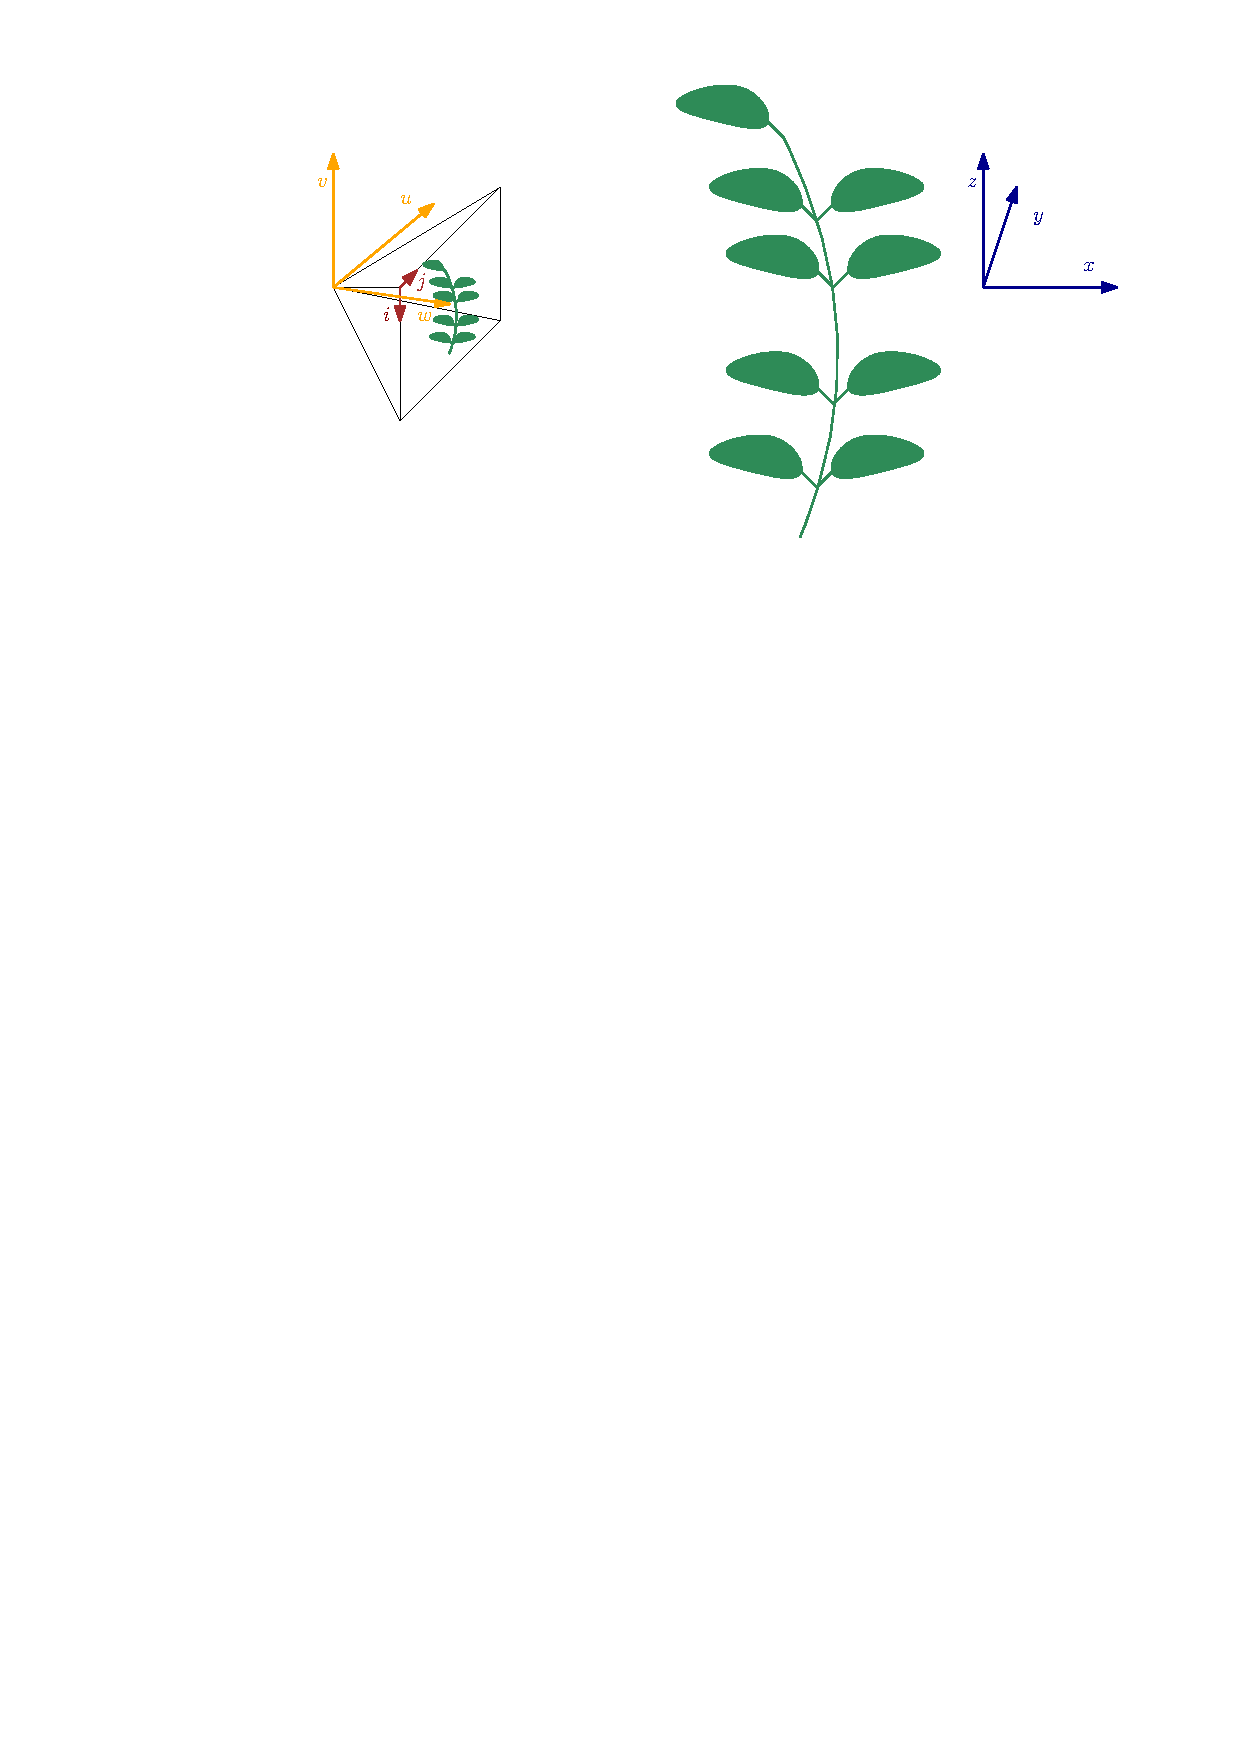
\includegraphics[width=0.7\textwidth]{images/reperes.pdf}

    Extrinsics: rotation $R$ and translation $T$.
    $$\left( \begin{array}{c}
    u \\ v \\ w
    \end{array} \right)= R\left( \begin{array}{c}
    x \\ y \\ z
    \end{array} \right) + T$$
\end{frame}

\begin{frame}{Fundamental matrix}
    \begin{columns}
        \begin{column}{0.4\textwidth}
            \centering
            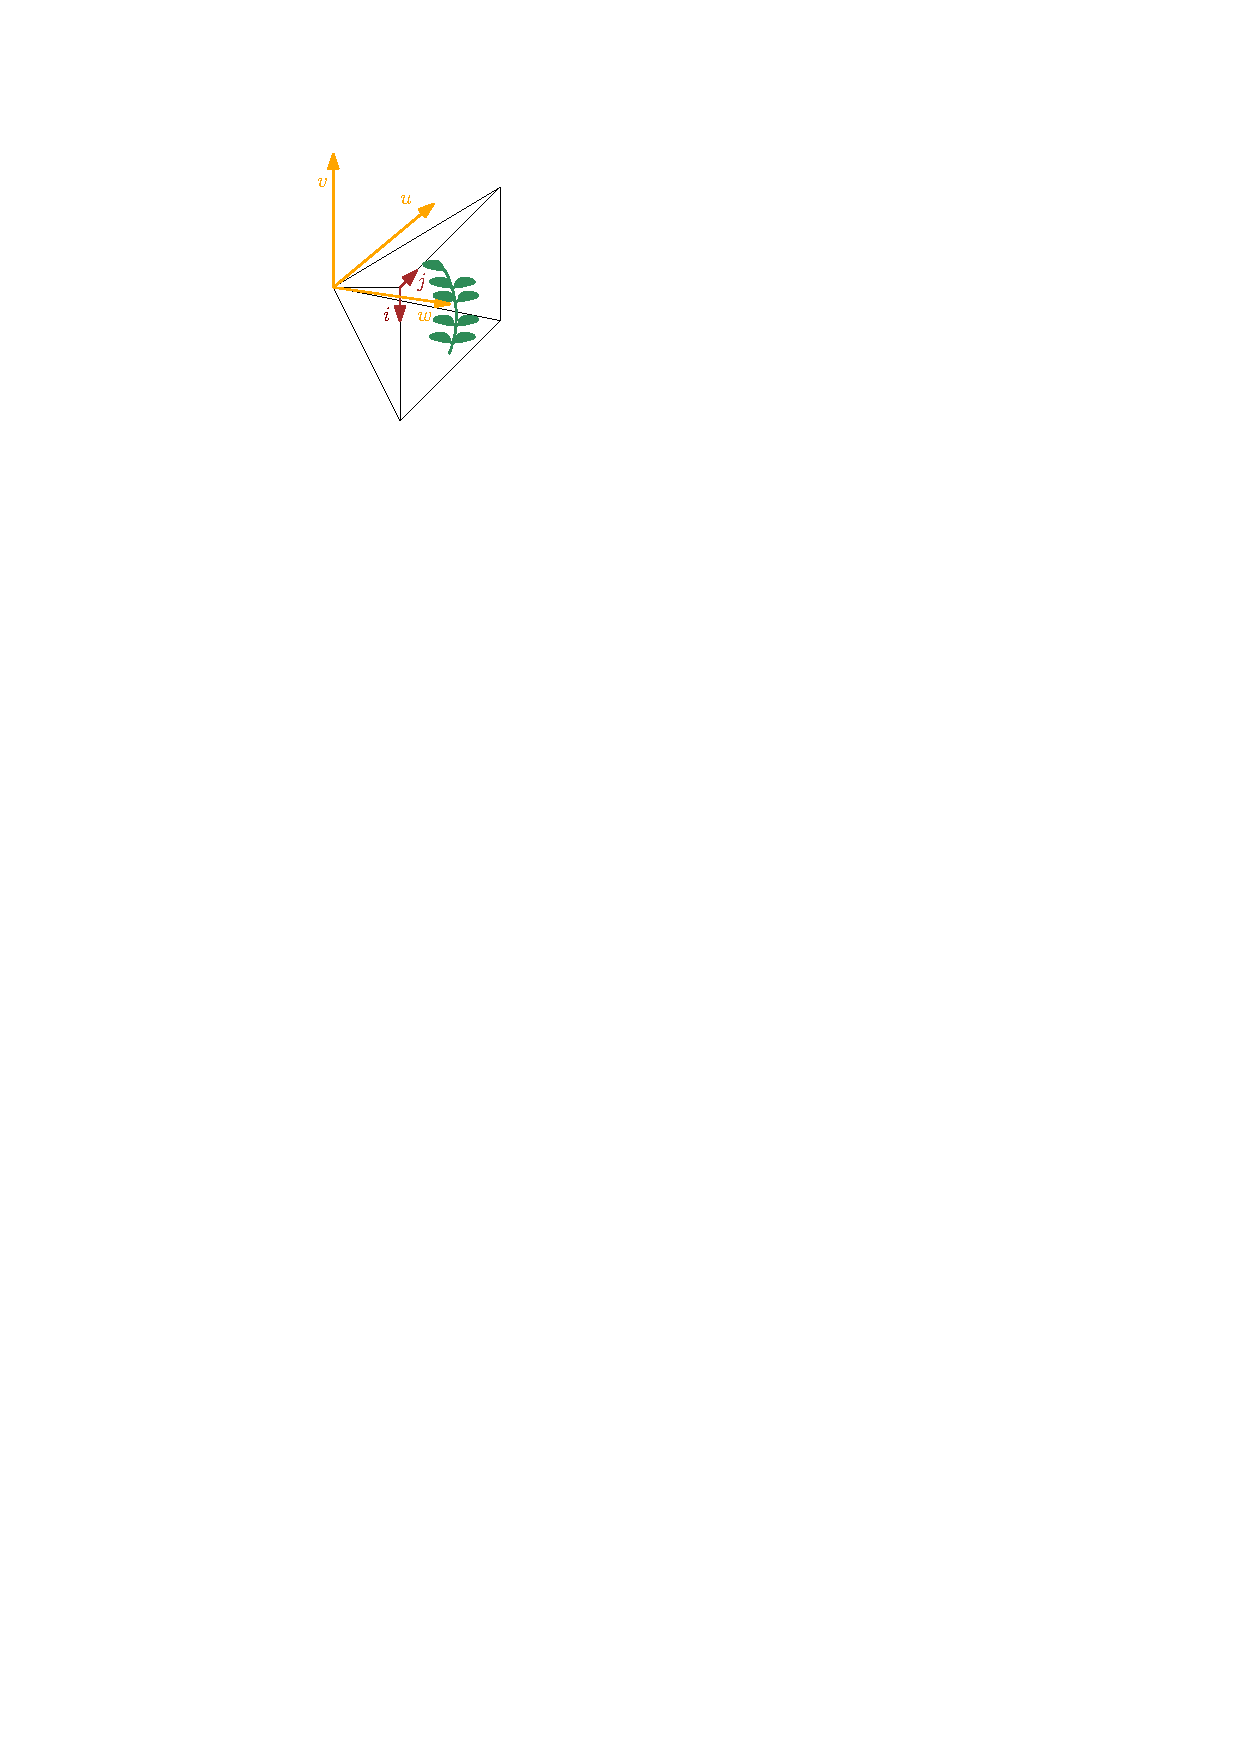
\includegraphics[width=\textwidth]{images/cam.pdf}
        \end{column}
        \begin{column}{0.6\textwidth}
            $$j = f_x \frac{u}{w} + c_x, i = f_y \frac{v}{w} + c_y$$

            $$\left( \begin{array}{c}
    j \\ i \\ 1
    \end{array} \right) = F \left( \begin{array}{c}
    u/w \\ v/w \\ 1
    \end{array} \right)$$ where

    $$F = \left( \begin{array}{ccc}
            f_x & 0 & c_x \\ 0 & f_y & c_y \\ 0 & 0 & 1
    \end{array} \right)$$
        \end{column}
    \end{columns}
\end{frame}

\begin{frame}{Pinhole camera model}
    \centering
    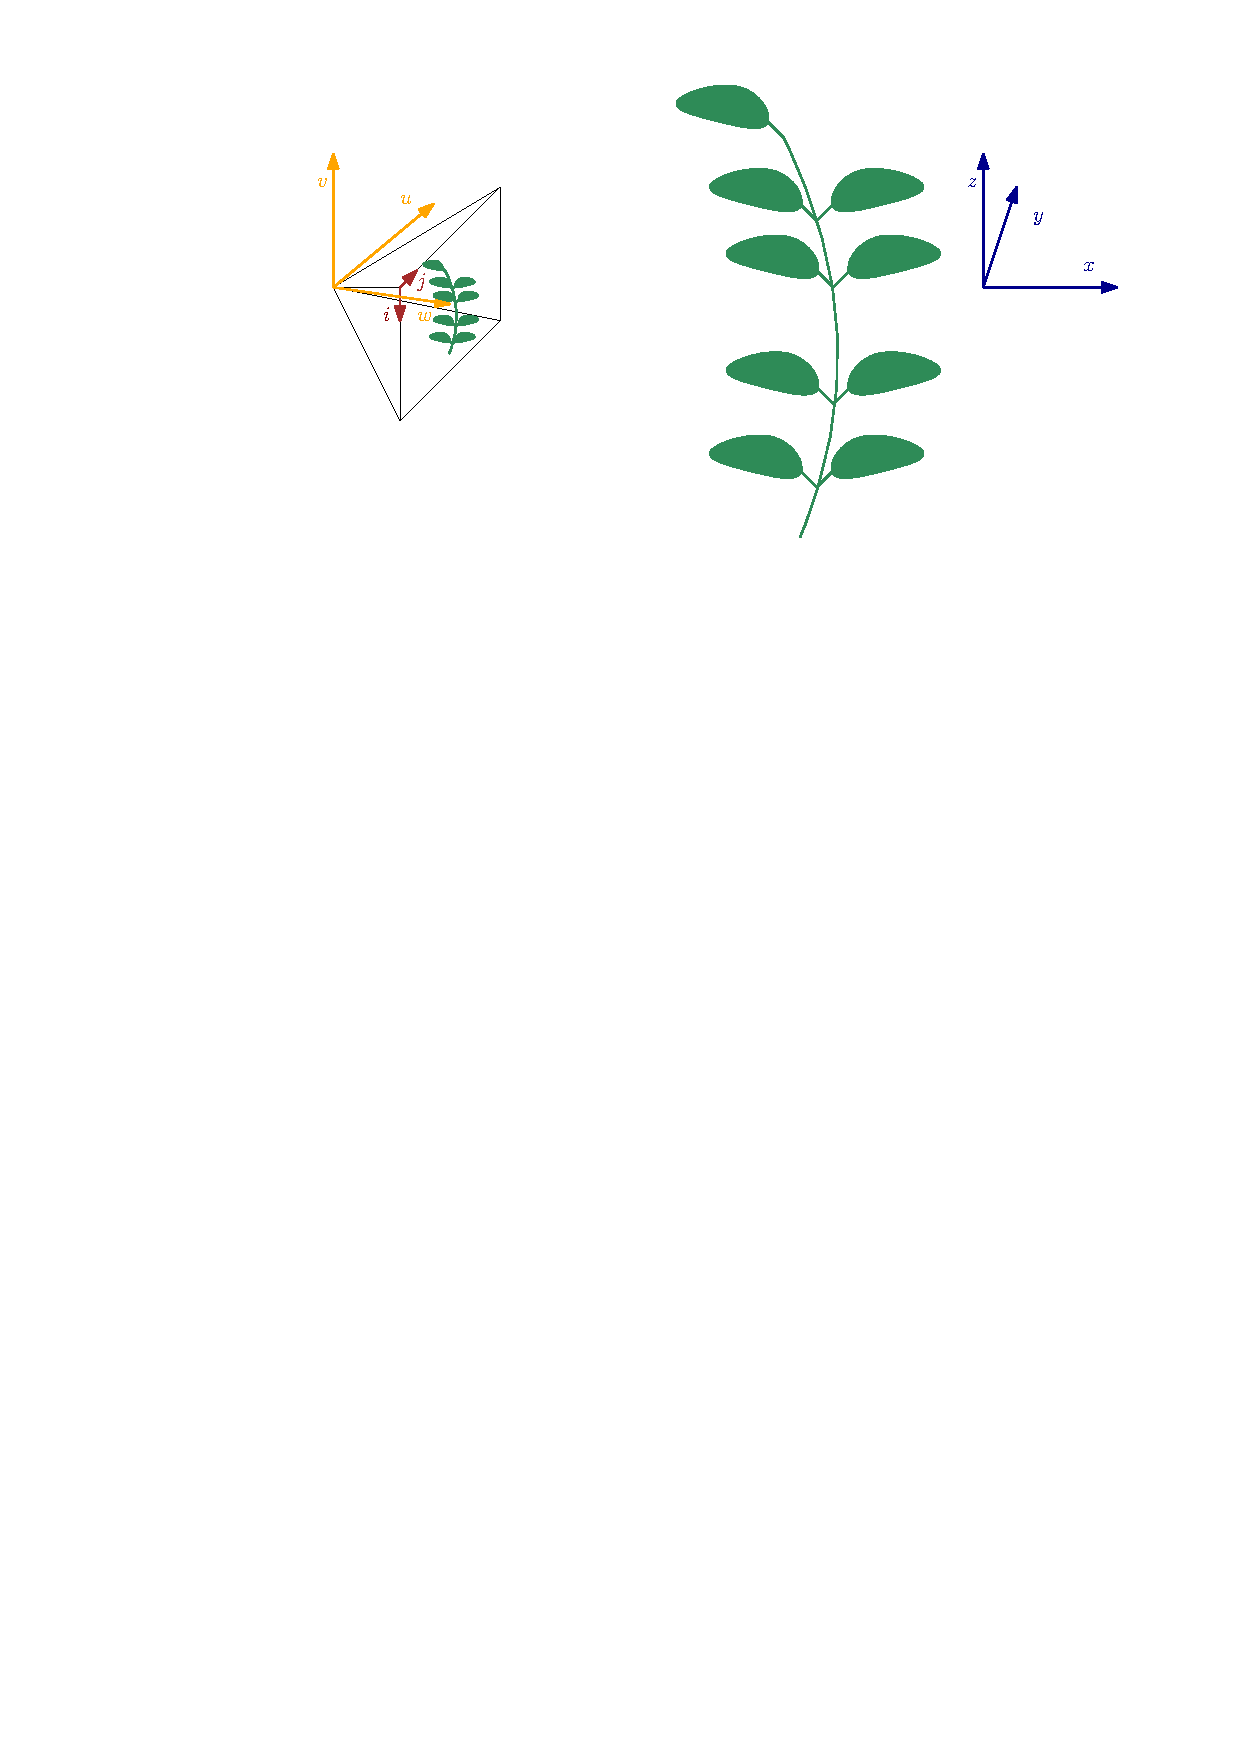
\includegraphics[width=0.6\textwidth]{images/reperes.pdf}

    Extrinsics: $\left( \begin{array}{c}
            u \\ v \\ w
            \end{array} \right)= R\left( \begin{array}{c}
            x \\ y \\ z
    \end{array} \right) + T$

    Intrinsics: $\left( \begin{array}{c}
            u \\ v \\ w
    \end{array} \right)$
\end{frame}
\begin{frame}{Camera distortion}
    \centering
    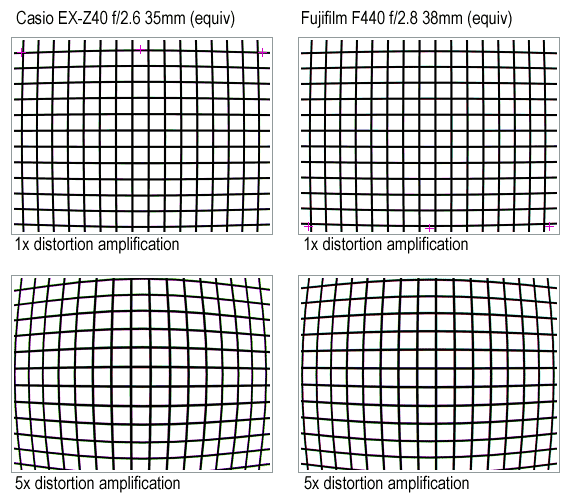
\includegraphics[width=0.3\textwidth]{images/qwe_download.png}
    \begin{block}{OpenCV model}
        \[
            r = \sqrt{x^2 + y^2}
        \]
        \[
            x_{\textrm{corrected}} = x(1+k_1r^2 + k_2r^4 + k_3r^6)
        \]
        \[
            y_{\textrm{corrected}} = x(1+k_1r^2 + k_2r^4 + k_3r^6)
        \]
        Simplified radial:
        $k_2 = k_3 = 0.$
    \end{block}

\end{frame}
\begin{frame}{Summary}
    \begin{block}{Camera parameters}
        5 to 7 parameters: $f_x, f_y, c_x, c_y, k_1, (k_2, k_3)$.
    \end{block}
    \begin{block}{Pose parameters}
        6 parameters: 3 for $R$, 3 for $T$.
    \end{block}
\end{frame}
\section{Stereo vision}
\begin{frame}
    \tableofcontents[sectionstyle=show/shaded]
\end{frame}
\begin{frame}{Basic principle}
    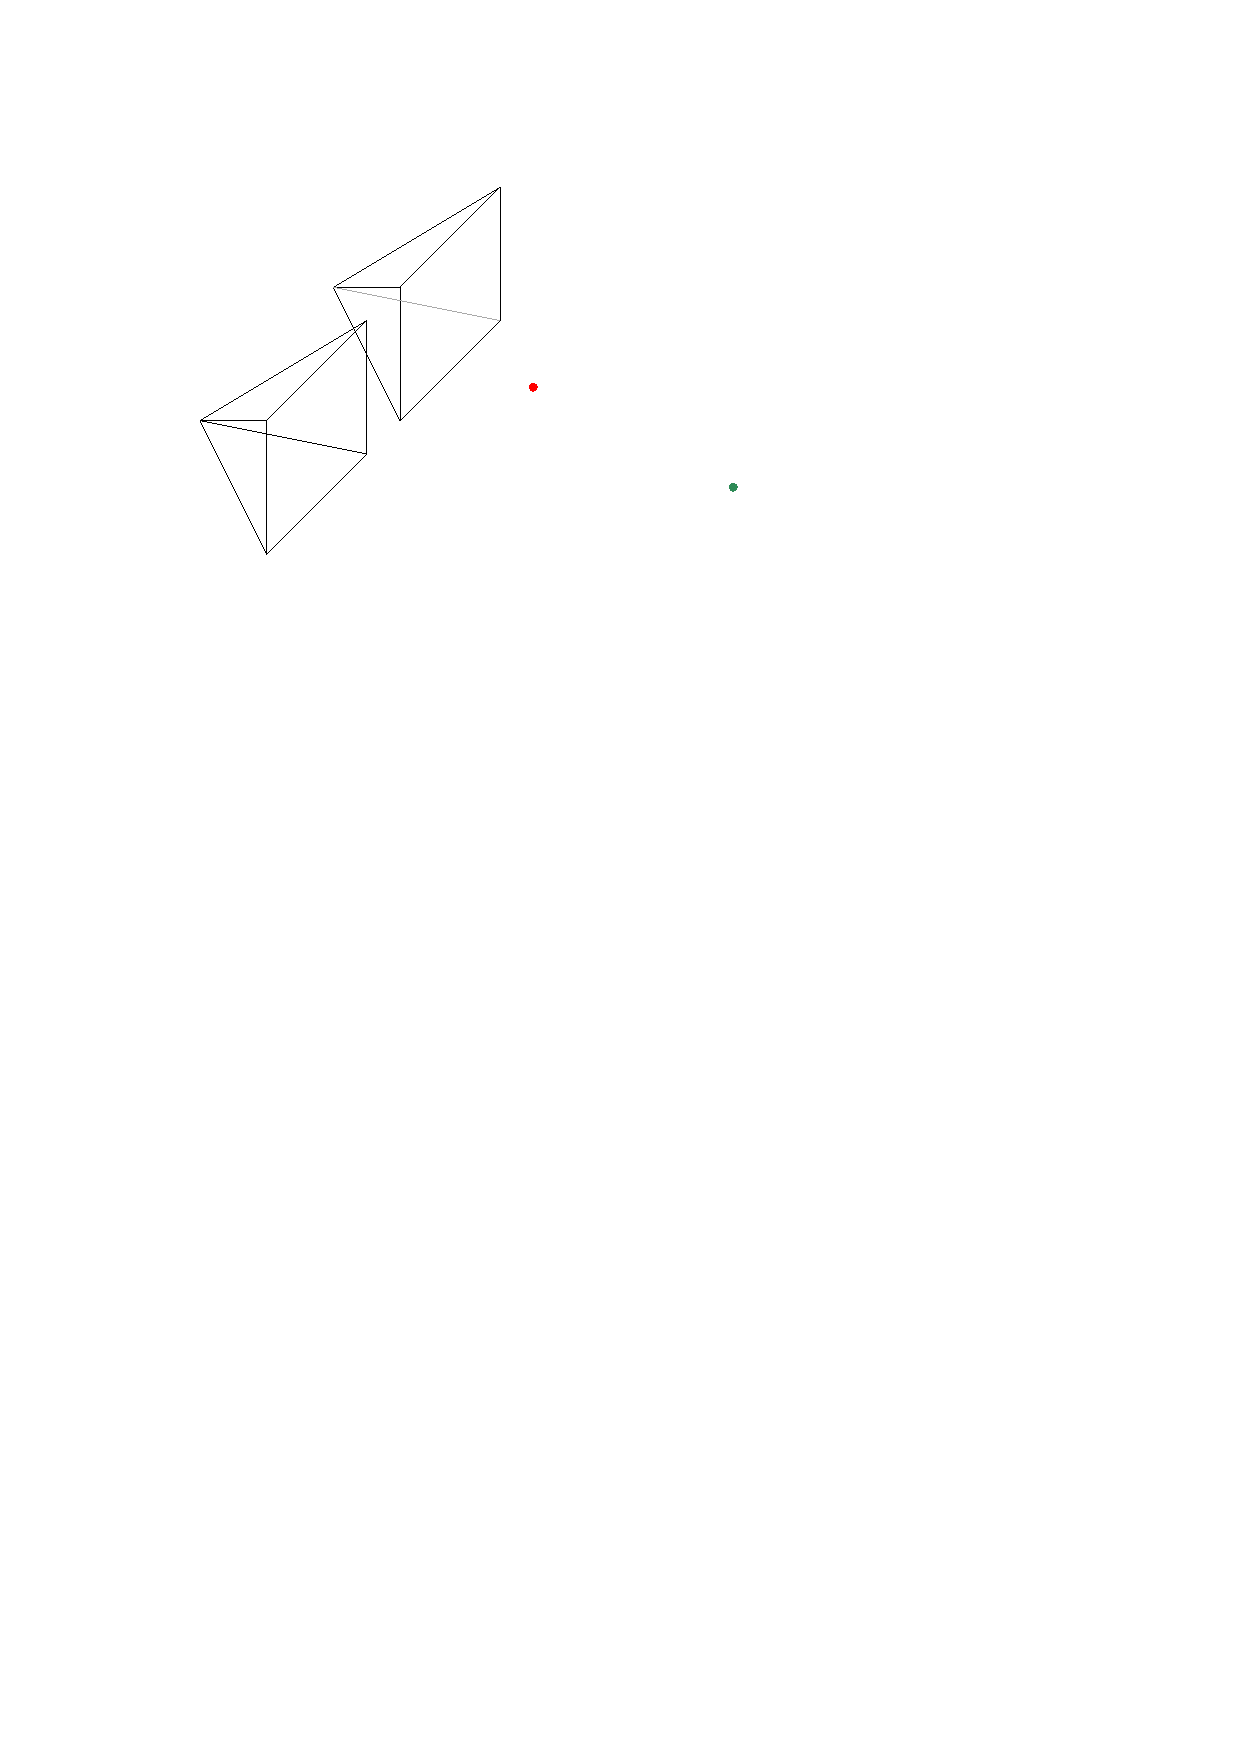
\includegraphics[width=\textwidth]{images/stereo.pdf}
\end{frame}

\begin{frame}{Basic principle}
    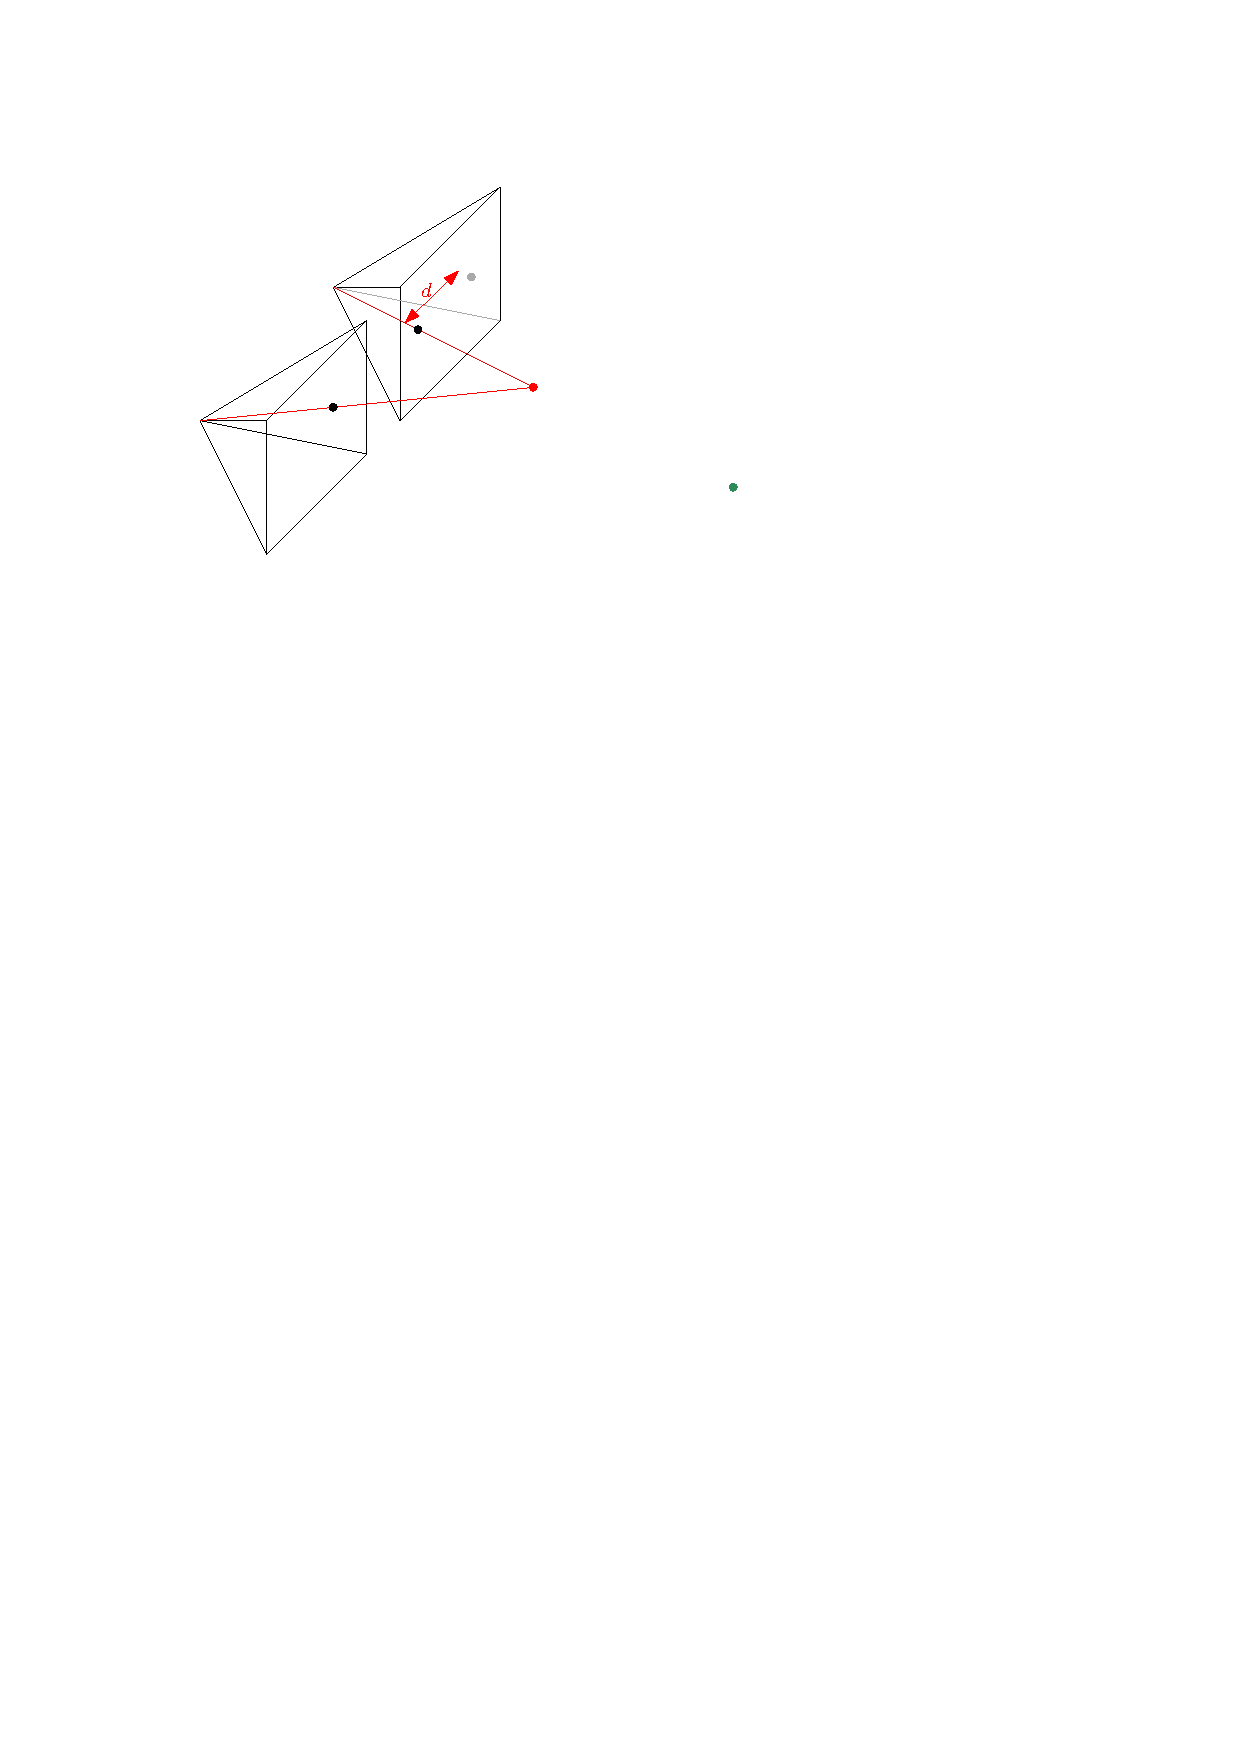
\includegraphics[width=\textwidth]{images/stereo_1.pdf}
\end{frame}

\begin{frame}{Basic principle}
    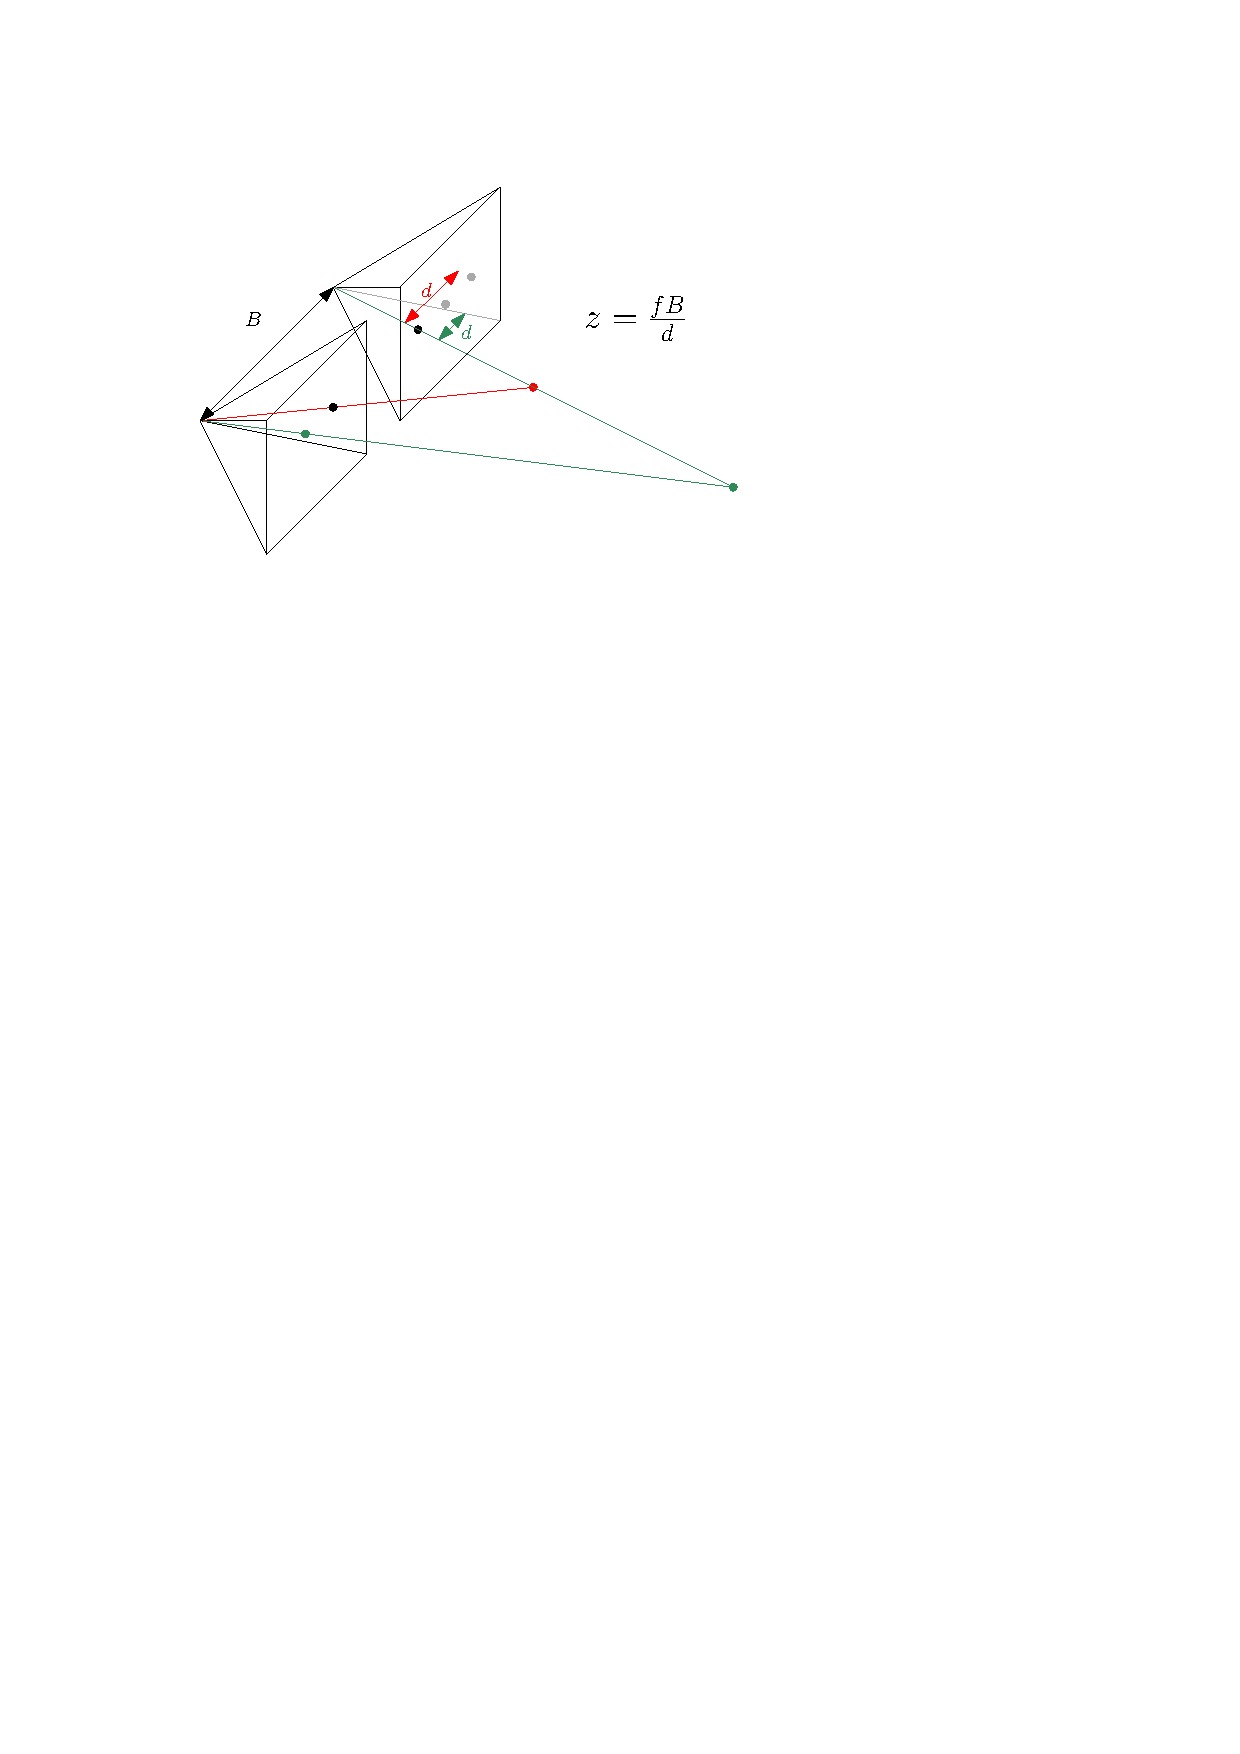
\includegraphics[width=\textwidth]{images/stereo_2.pdf}
\end{frame}


\begin{frame}{Disparity map}
    \begin{block}{Goal}
        Compute $d$ at every point in the image.
    \end{block}
    \vspace{1em}
    \centering
    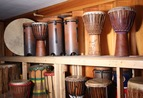
\includegraphics[width=0.3\textwidth]{images/im0.jpg}
    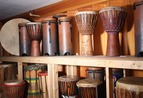
\includegraphics[width=0.3\textwidth]{images/im1.jpg}
    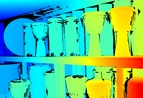
\includegraphics[width=0.3\textwidth]{images/disp0.jpg}
\end{frame}

\section{Photogrammetry}
\begin{frame}
    \tableofcontents[sectionstyle=show/shaded]
\end{frame}
\begin{frame}{Principle}
    \begin{columns}
        \begin{column}{0.45\textwidth}
            \centering
            RGB Images

            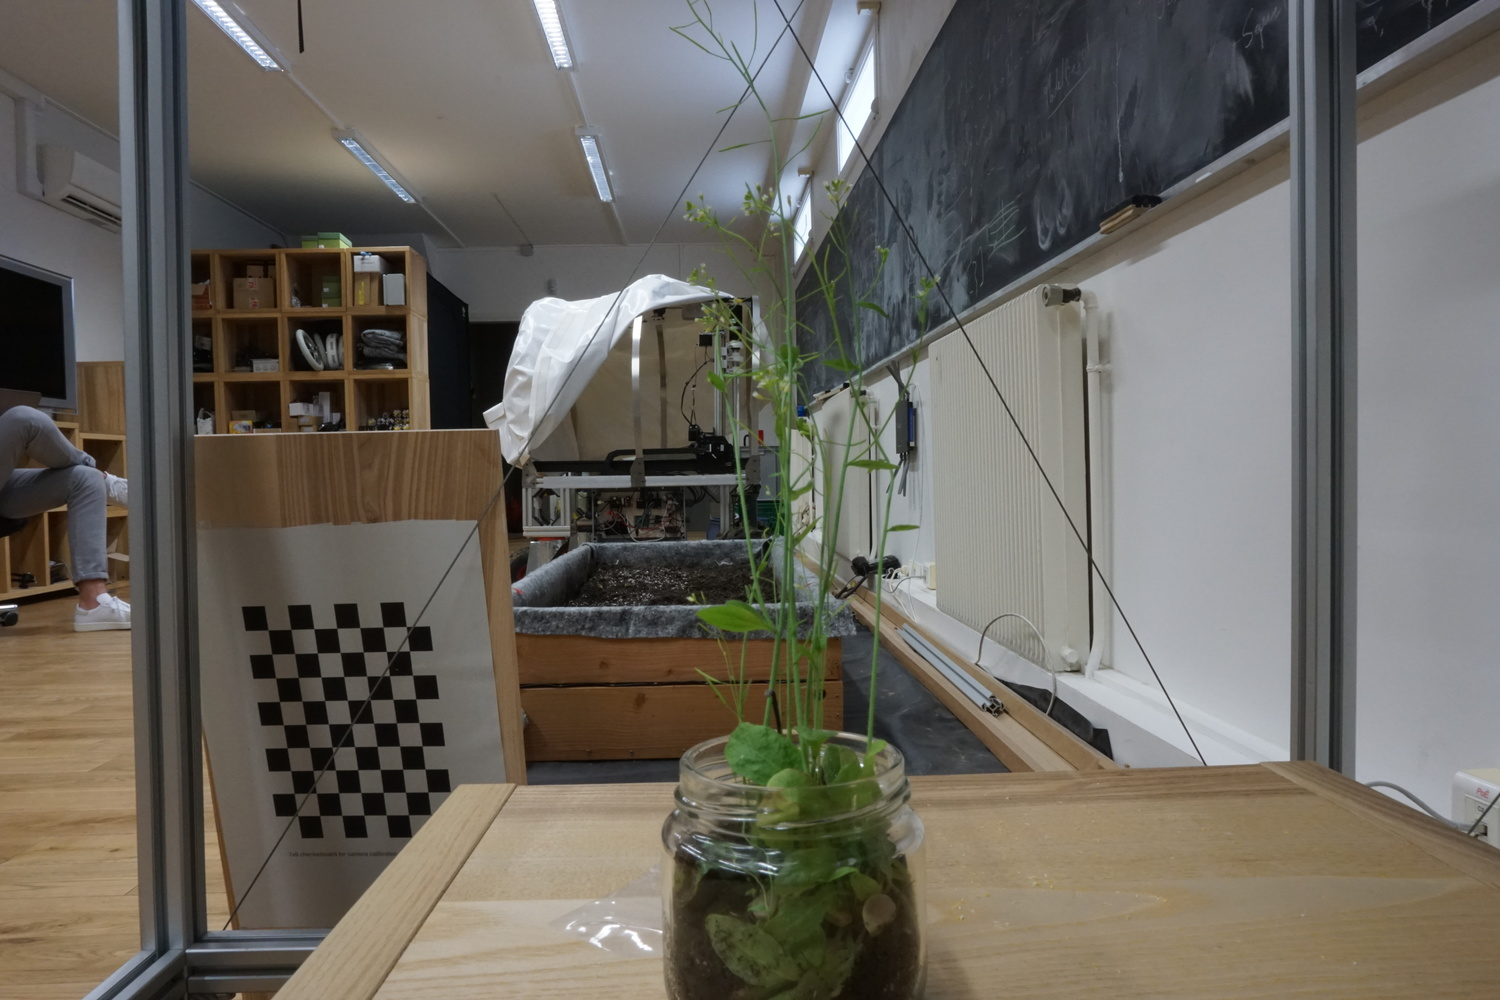
\includegraphics[width=0.3\textwidth]{images/rgb000.jpg}
            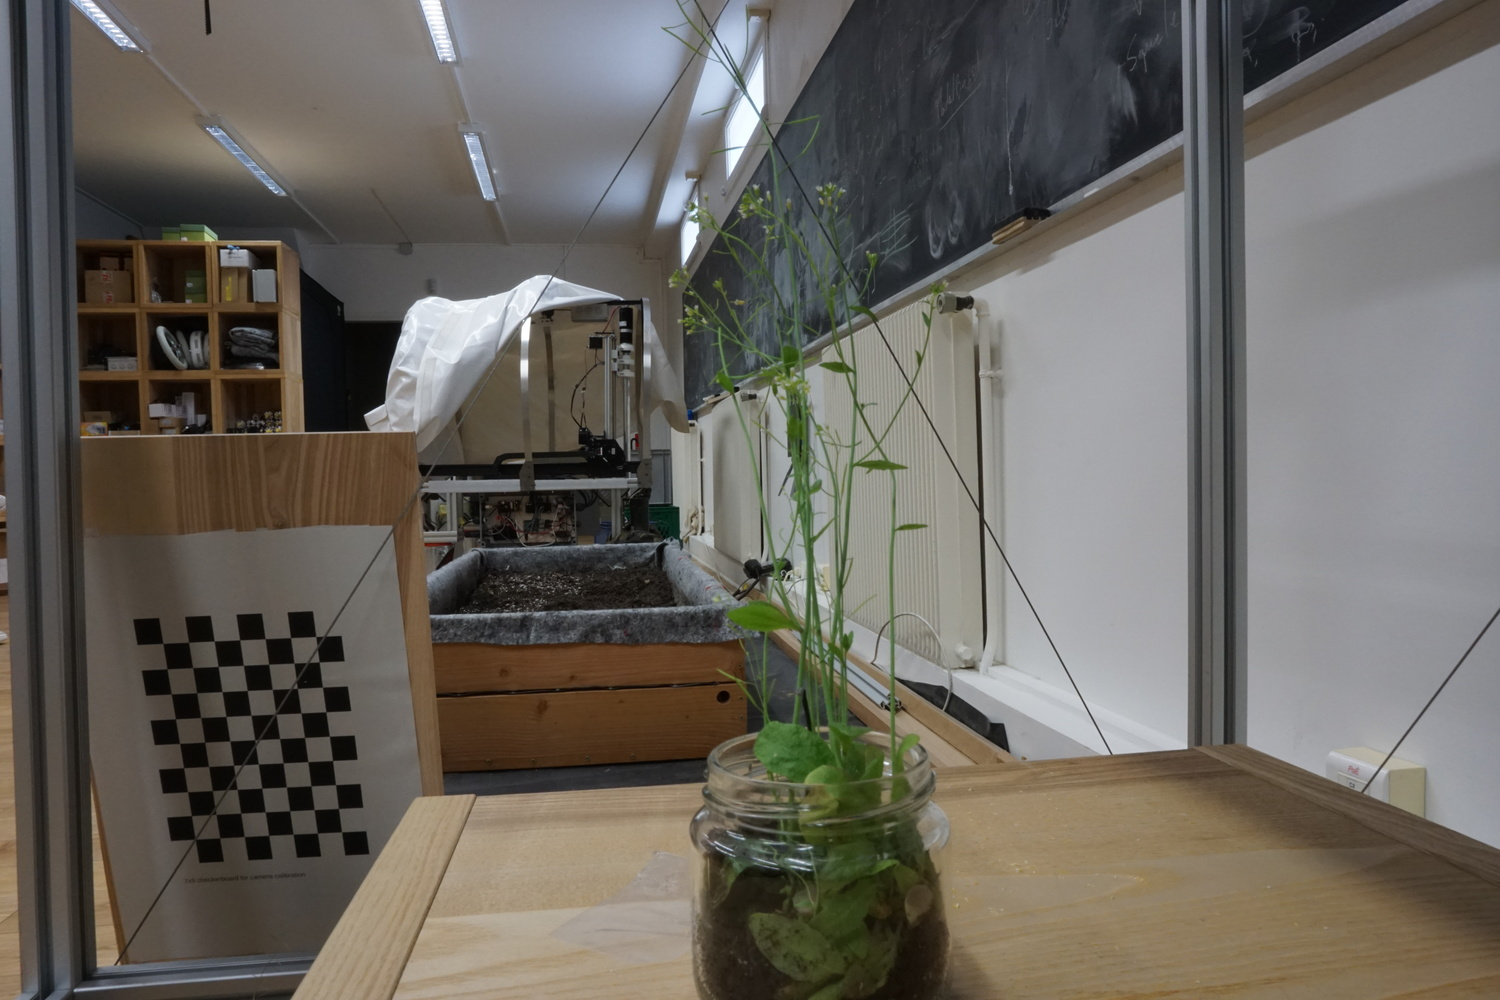
\includegraphics[width=0.3\textwidth]{images/rgb001.jpg}
            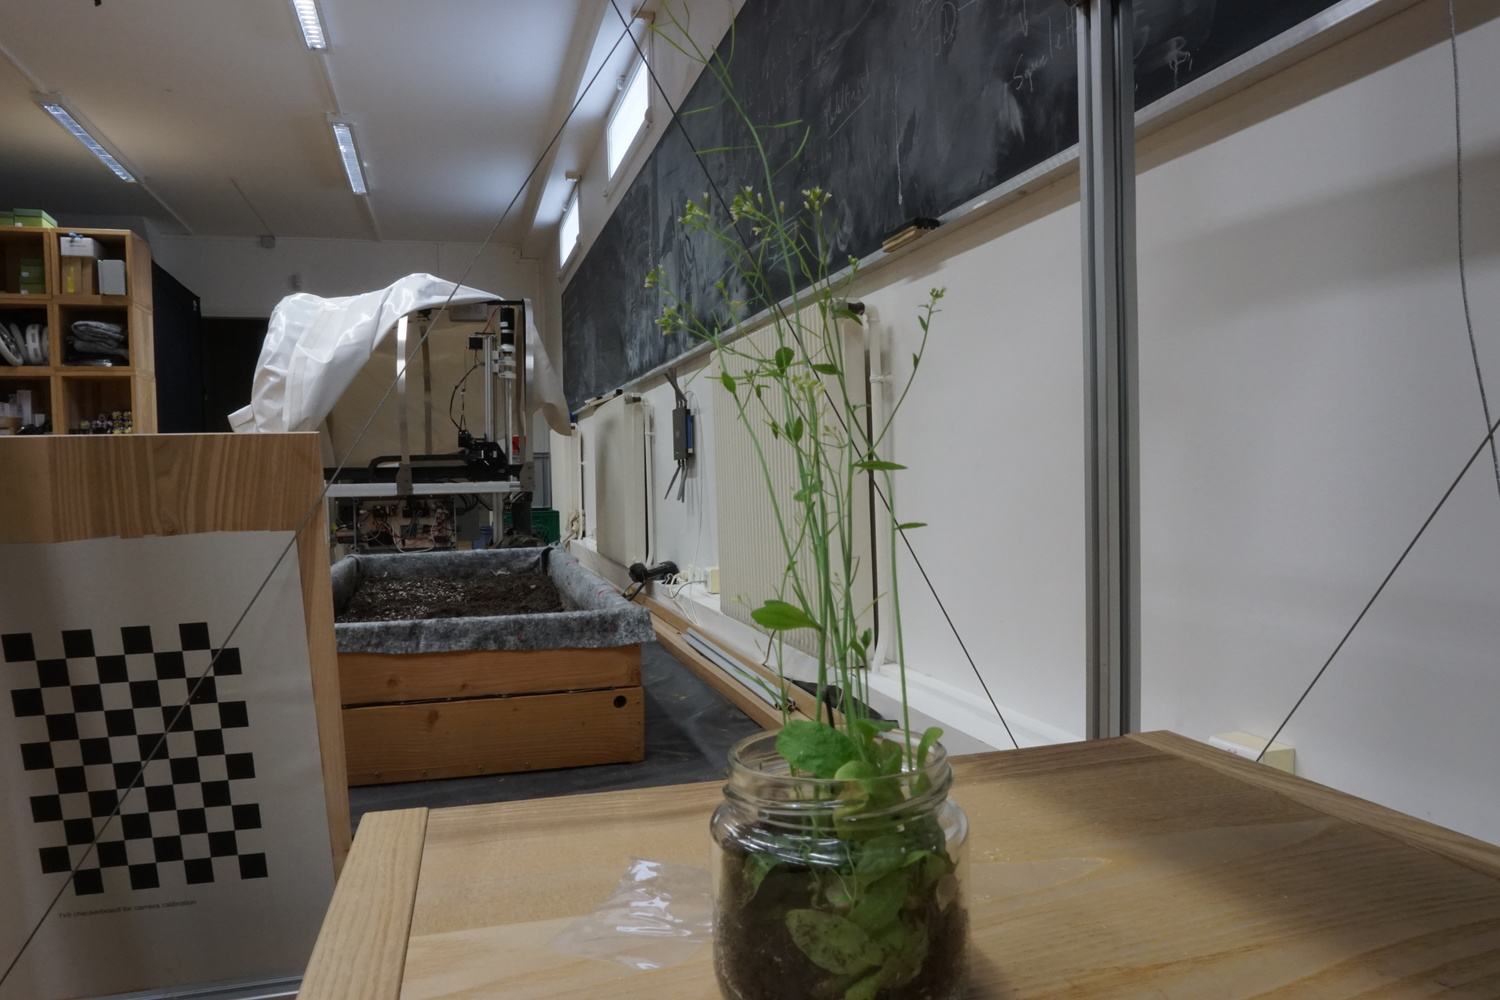
\includegraphics[width=0.3\textwidth]{images/rgb002.jpg}
            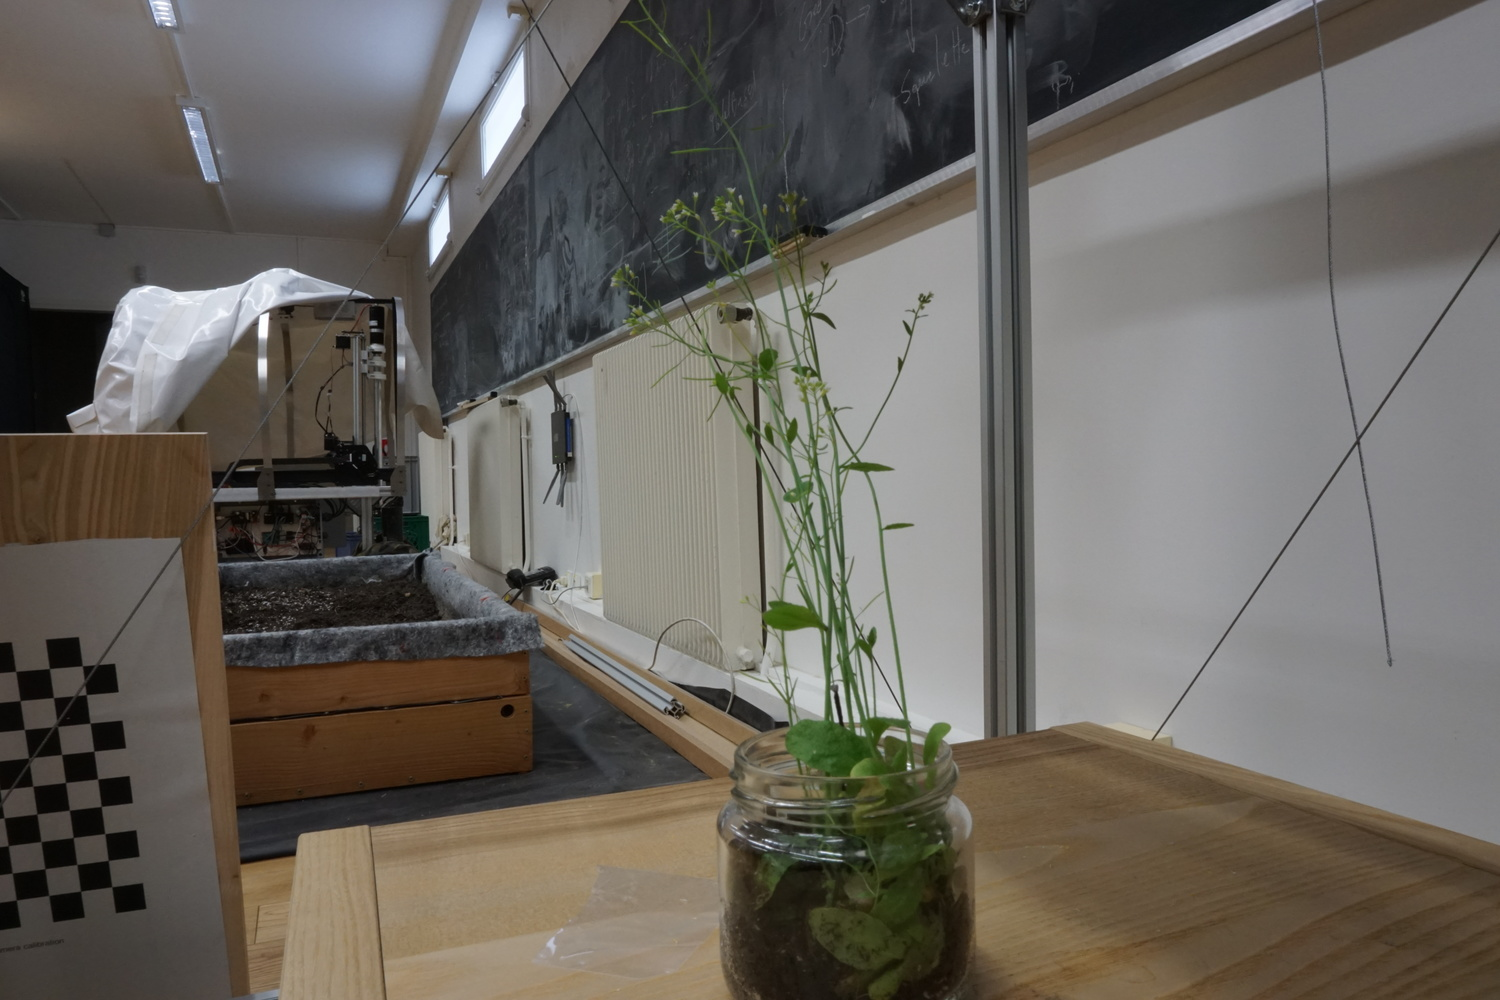
\includegraphics[width=0.3\textwidth]{images/rgb003.jpg}
            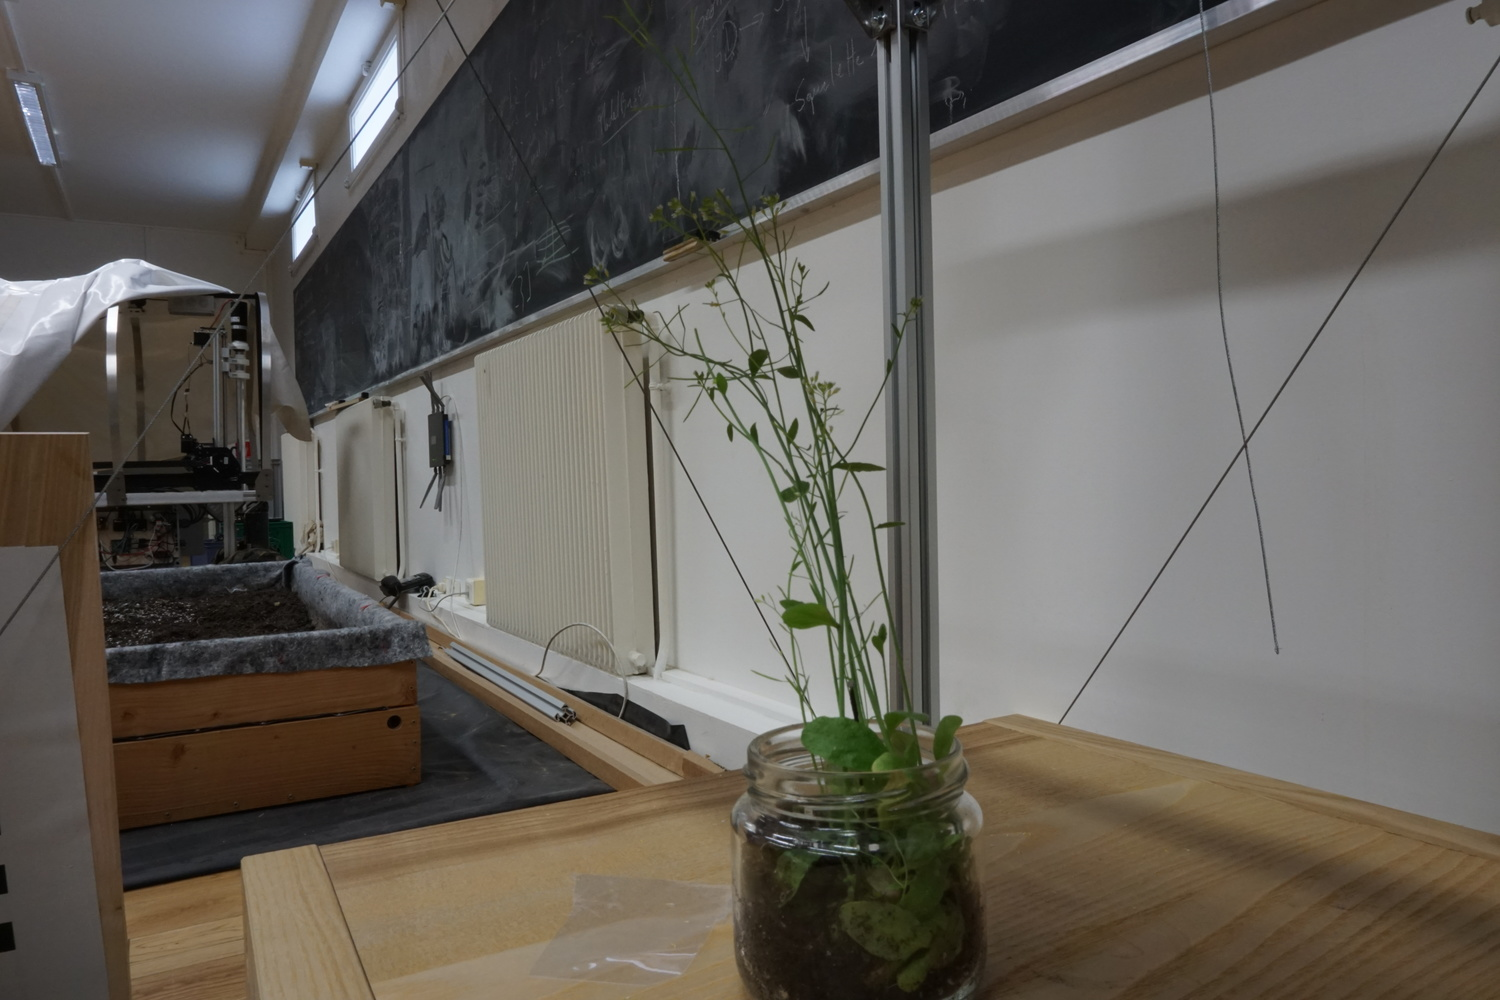
\includegraphics[width=0.3\textwidth]{images/rgb004.jpg}
            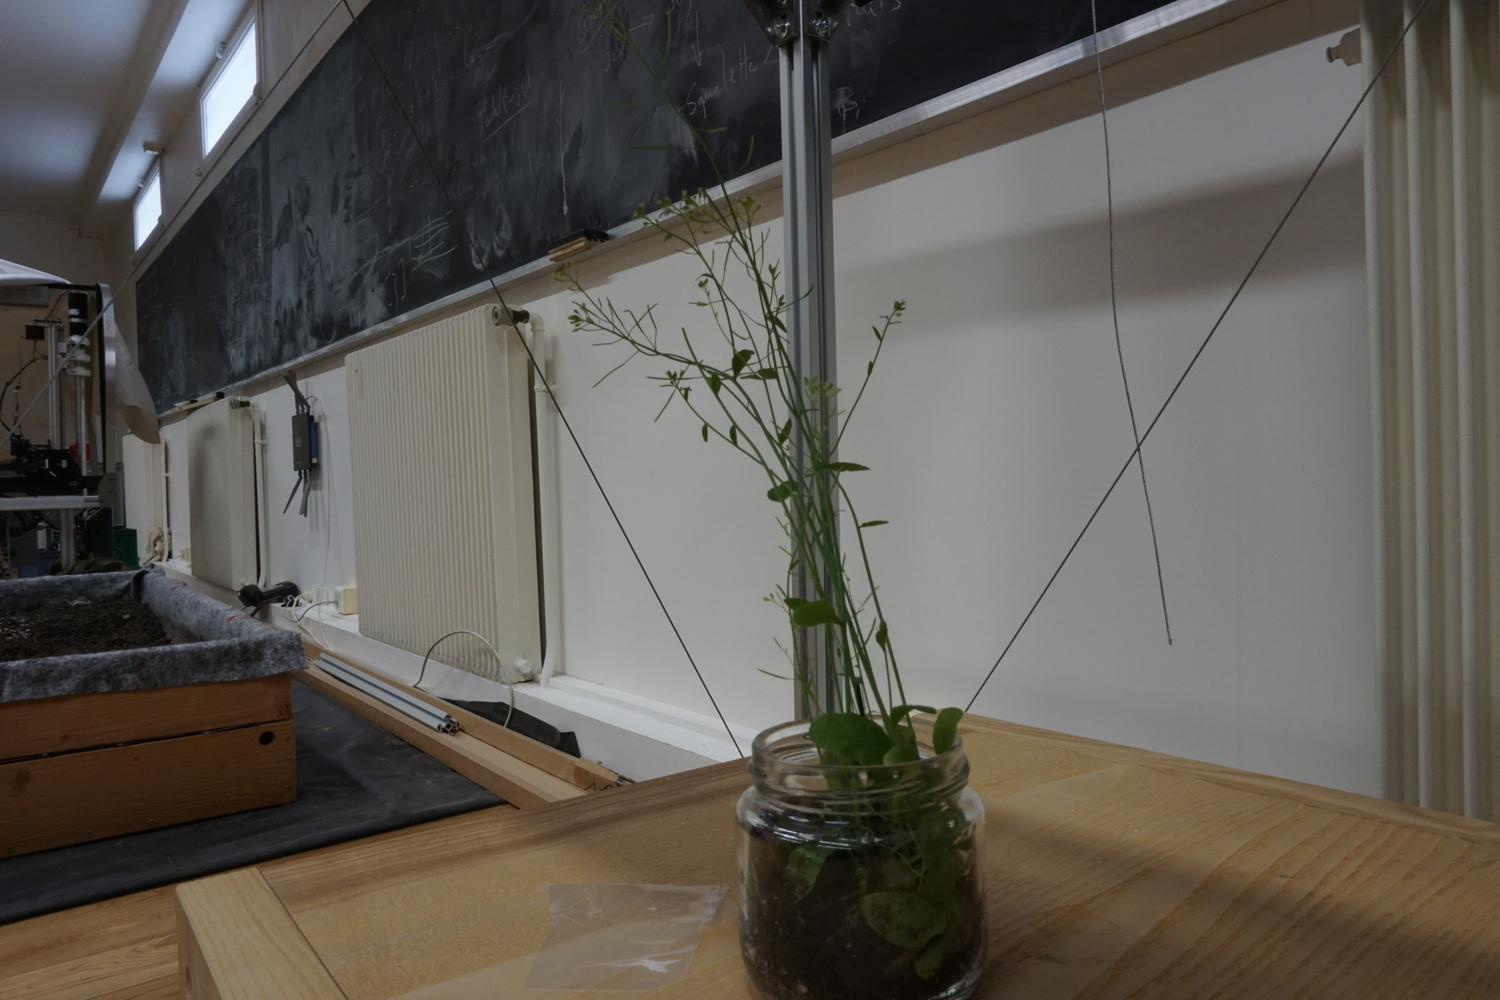
\includegraphics[width=0.3\textwidth]{images/rgb005.jpg}
            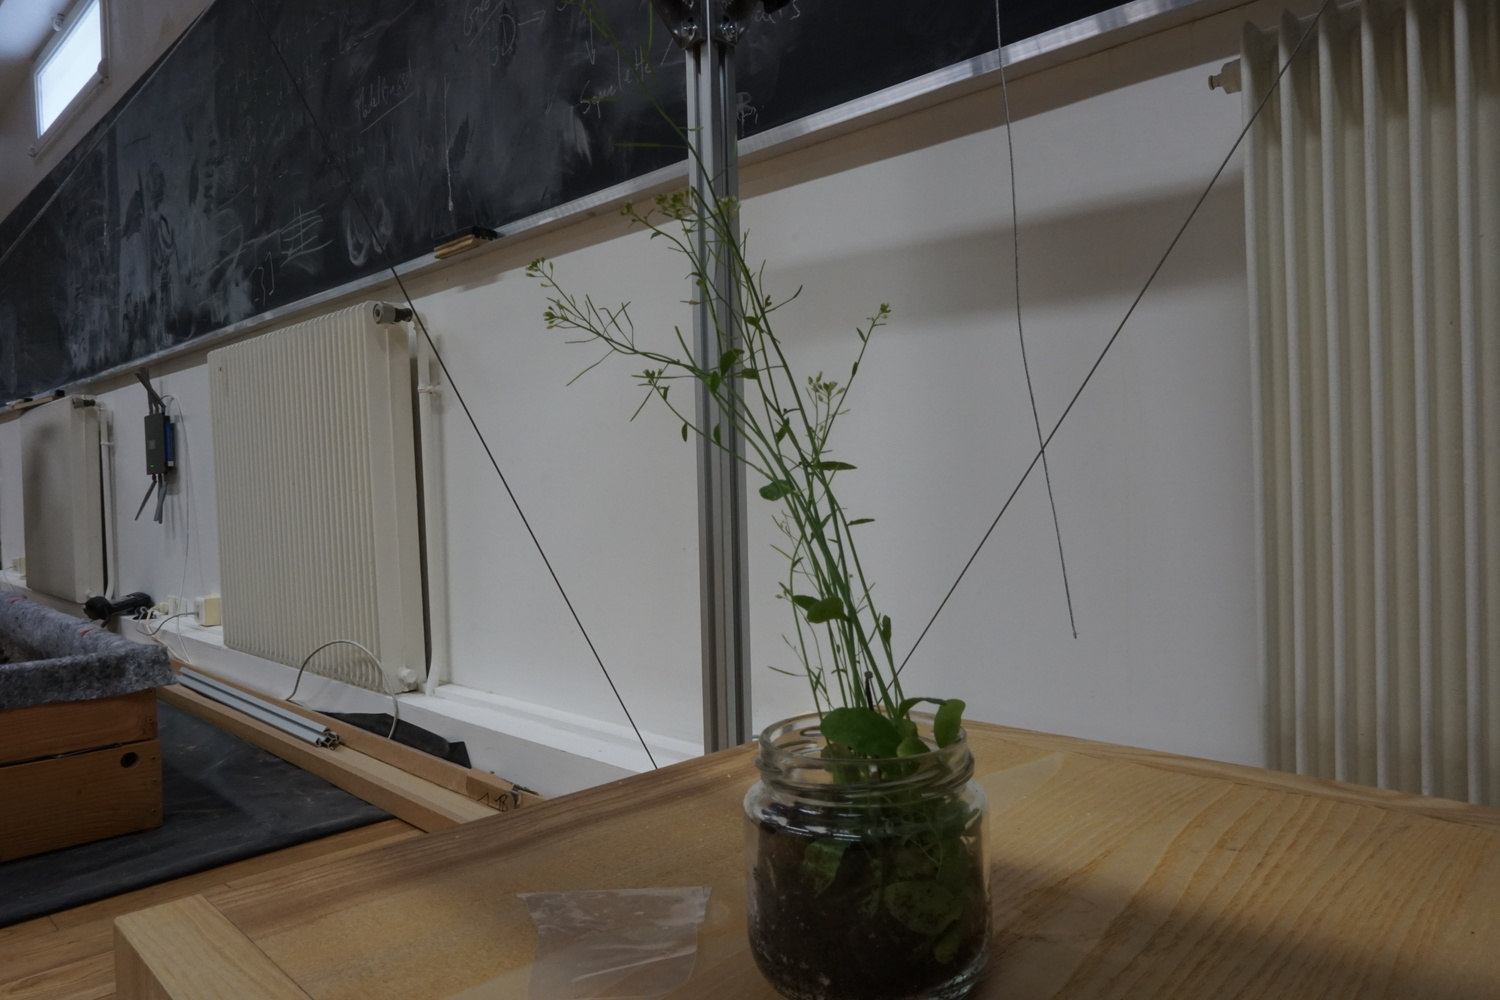
\includegraphics[width=0.3\textwidth]{images/rgb006.jpg}
            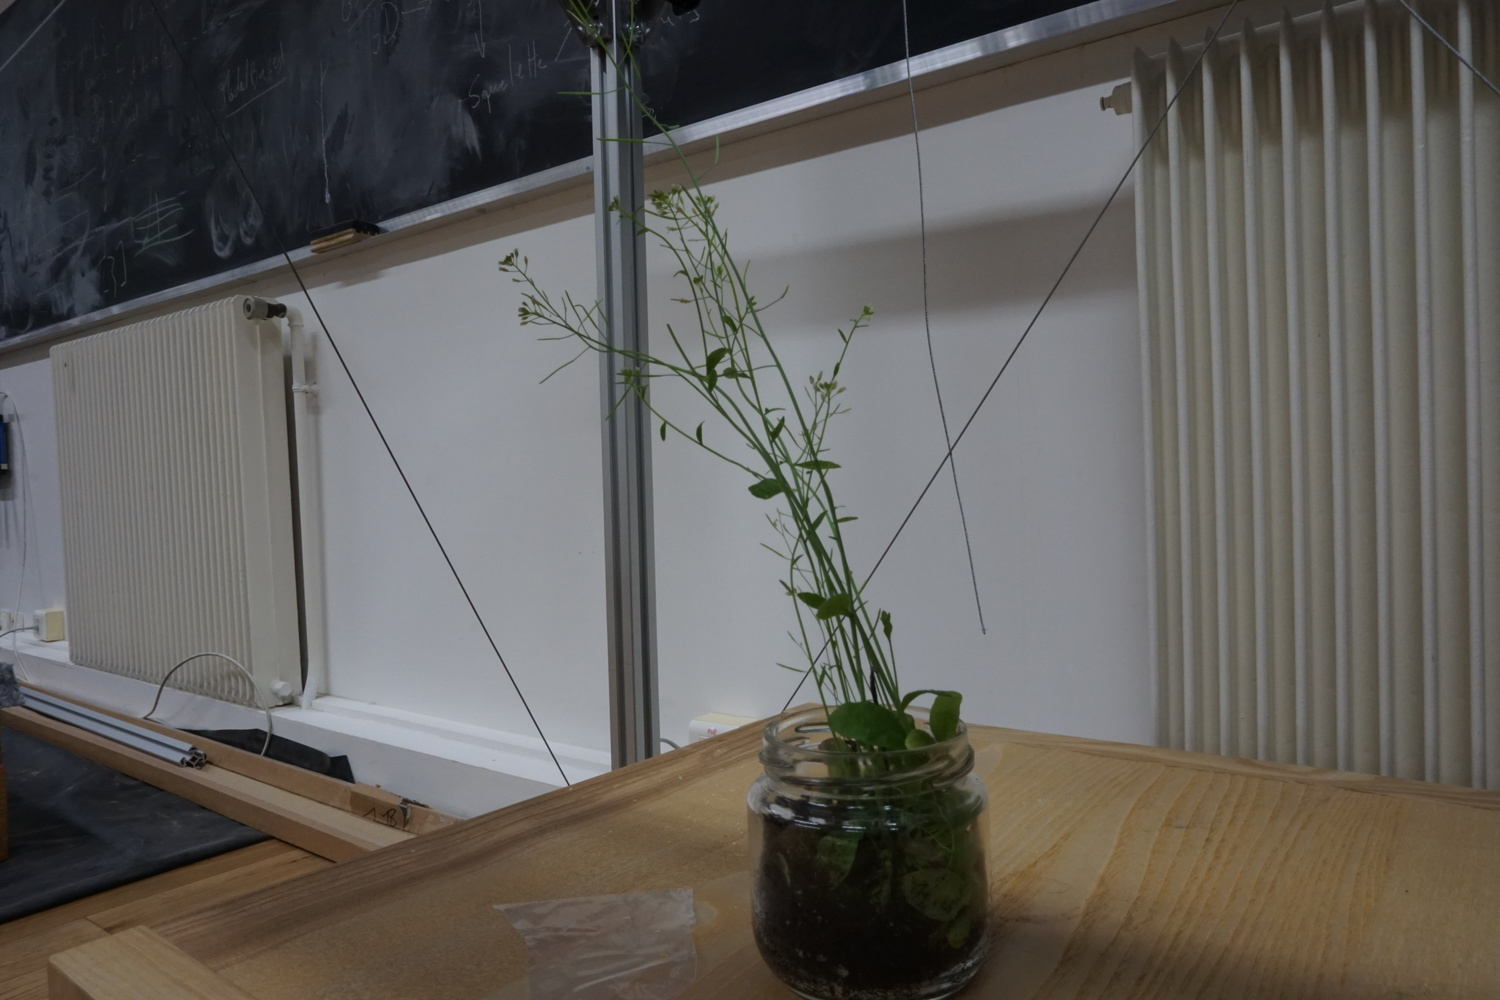
\includegraphics[width=0.3\textwidth]{images/rgb007.jpg}
            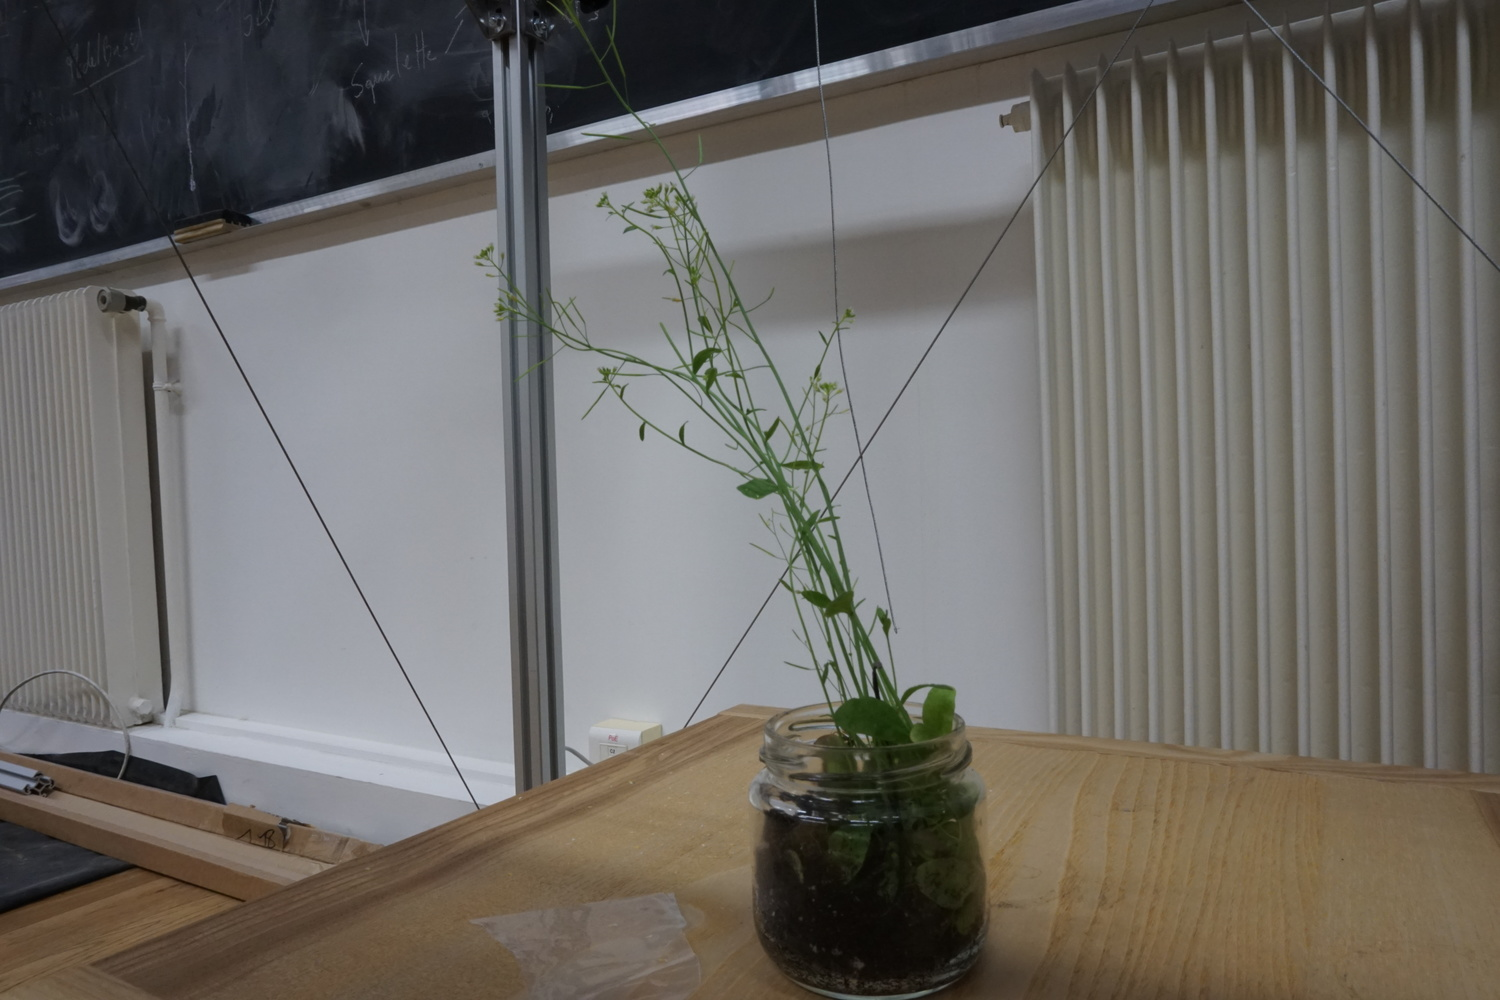
\includegraphics[width=0.3\textwidth]{images/rgb008.jpg}
        \end{column}
        \begin{column}{0.1\textwidth}
$\Rightarrow$
        \end{column}
        \begin{column}{0.45\textwidth}
            \centering
            Point Cloud

             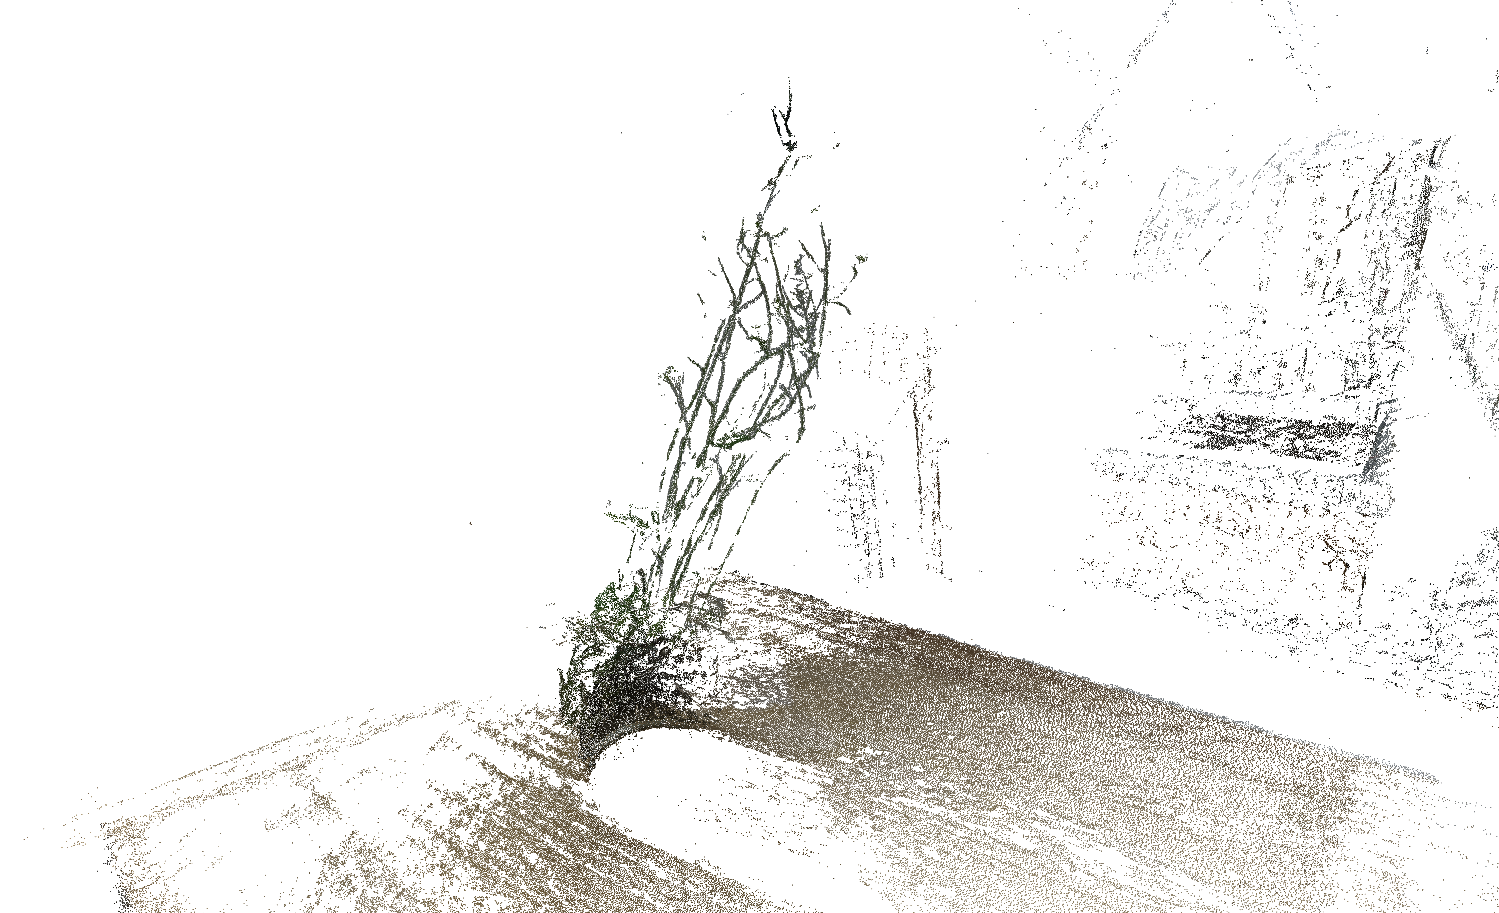
\includegraphics[width=\textwidth]{images/pointcloud.png}
        \end{column}
    \end{columns}
        \vspace{2em}
    \begin{block}{Solutions}
        Free and open source: colmap, openMVG+openMVS, \dots

        Commercial: agisoft, \dots

    \end{block}
\end{frame}
\begin{frame}{Pipeline}
    \begin{itemize}
        \item Feature detection and computation
        \item Feature matching
        \item Pose estimation
        \item Bundle adjustment
        \item Dense point cloud generation
    \end{itemize}
\end{frame}
\begin{frame}{Feature detection and matching}
    \centering
         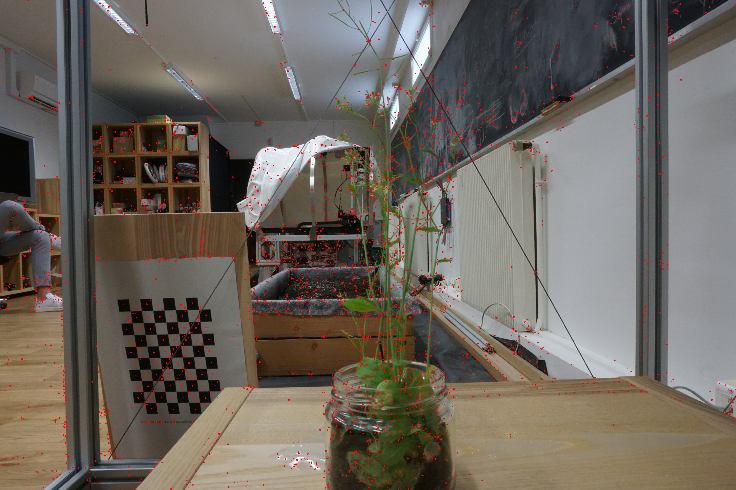
\includegraphics[width=.5\textwidth]{images/sift.png}
         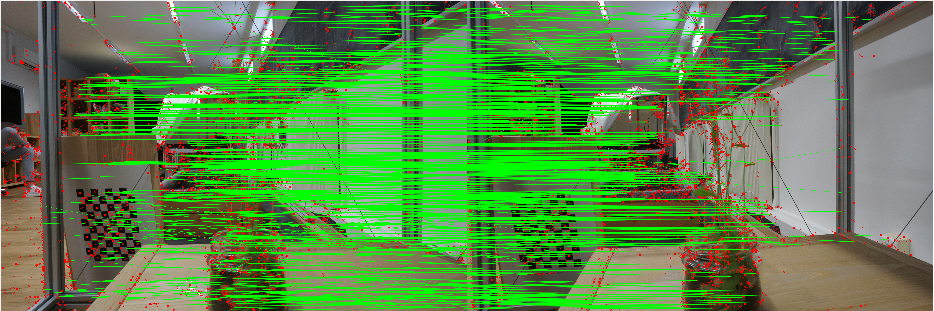
\includegraphics[width=\textwidth]{images/matches.png}
\end{frame}
\begin{frame}{Pose estimation}
    For every match of a real world point $\mathbf{x} = (x, y, z)$, between a camera pair $k_1, k_2$. Let $x_1 = (i_1, j_1)$ be the pixel in view $k_1$, and $x_2 = (i_2, j_2)$ be the corresponding pixel in view $k_2$. We get the equations:

    $$F(R_1 \mathbf{x} + T_1) = \mathbf{x}_1$$
    $$F(R_2 \mathbf{x} + T_2) = \mathbf{x}_2$$

    For every match, we add 4 equations and 3 unknowns. With enough matches, we can recover the relative pose of the two views up to a homotopy of the whole space.
\end{frame}
\begin{frame}{Pose estimation}
    Iterating this over all pairs of images we obtain:
    \begin{itemize}
        \item The relative pose of all cameras.
        \item A sparse set of 3D points corresponding to the matches.
    \end{itemize}
\end{frame}
\begin{frame}{Bundle adjustment}
    Refine the pose of all cameras and the position of all points simultaneously:

    \[
        \min_{R_i, T_i, F, x_i} \sum_i \sum_j v_{i,j} d(F(R_i x_i + T_i), y_i)^2,
    \]
    where:
    \begin{itemize}
        \item $R_i, T_i, F$: camera parameters,
        \item $x_i$: 3D points,
        \item $d$: euclidian distance.
    \end{itemize}
\end{frame}
\begin{frame}{Result (colmap)}
    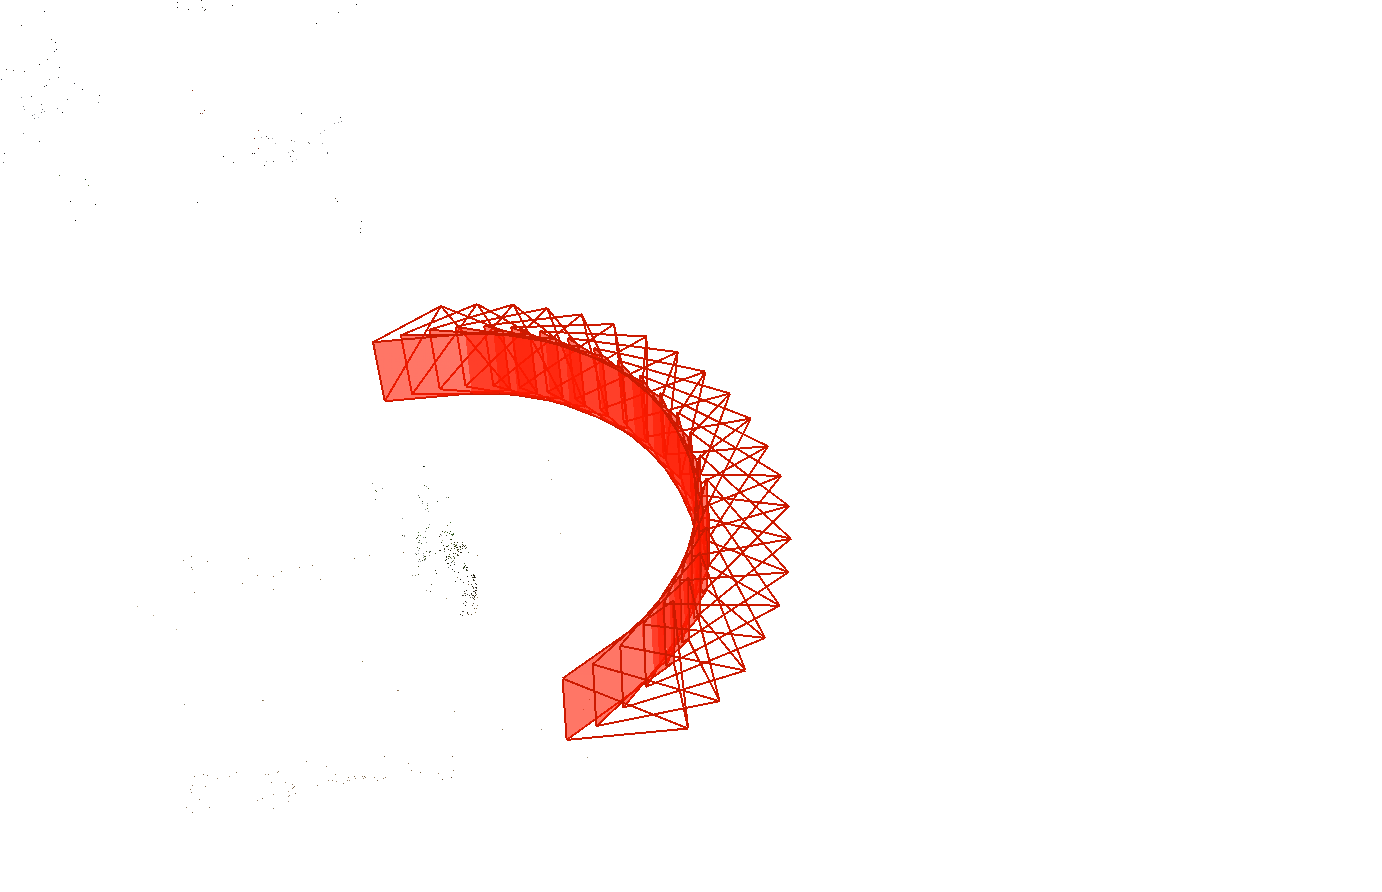
\includegraphics[width=\textwidth]{images/poses.png}
\end{frame}
\begin{frame}{Dense point cloud}
    We compute stereo disparity maps in each pair of images:
    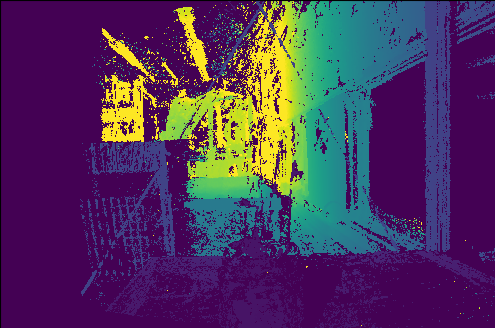
\includegraphics[width=\textwidth]{images/depthmap.png}
\end{frame}
\end{document}
